\section{Analysis and discussion}

In the following, the uncertainties of all measurement data, measured values and measurement results are determined according to GUM\cite{gum}.

\subsection{Mean lifetime of muons}

First, the mean lifetime of muons is supposed to be determined.
In order to do so, it is necessary to set a time calibration so that the channel number $K$ can be rewritten as time $t$.
This time calibration can be done by looking at the recorded pulse spectrum, which shows a periodical set of $15$ sharp peaks with a constant time distance of $\Delta t=0.64\,\mu$s between two directly adjacent peaks.
A gaussian fit of the shape
\begin{align} \label{Gaussian}
f(x)=A\cdot\exp\left( -\frac{(x-\mu)^2}{2\sigma ^2}\right) + B
\end{align}
\noindent is applied to each of the $15$ peaks to get their exact positions $\mu$ in the range of the channels $K$.
Now, integer multiple of the time distance or rather time interval $\Delta t$ are plotted against these peak positions, which leads to the diagram in figure \ref{TimeCalibration}.
\begin{figure}[H]
	\centering
	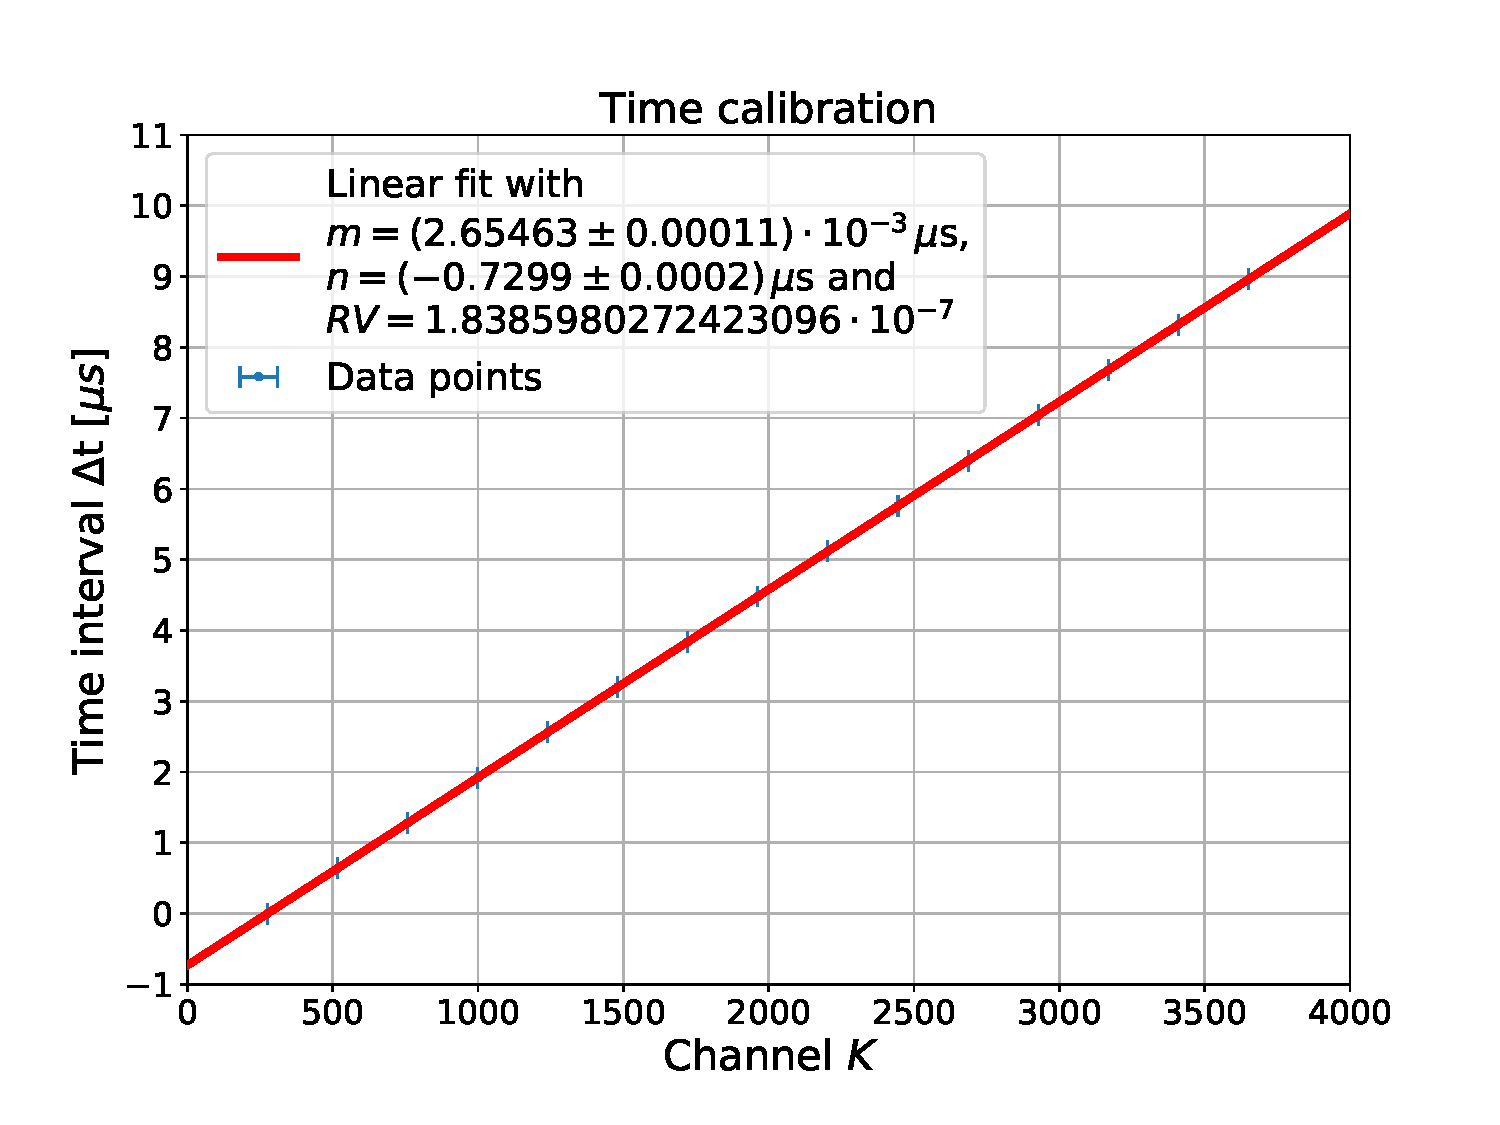
\includegraphics[width=0.8\textwidth]{src/TimeCalibration}
	\caption{This figure shows the diagram, which is used for the time calibration.}
	\label{TimeCalibration}
\end{figure}
\noindent In this process, the first peak of the pulse spectrum is interpreted as zero.
If you look at the diagram and the distribution of the data points, you can see a linear increase.
That's why a linear fit of the shape 
\begin{align} \label{line}
g(x)=m\cdot x + n
\end{align}
\noindent is applied.
This fit curve and its parameters can be seen in the diagram and its legend in figure \ref{TimeCalibration}.
With these results the channel number $K$ of a time spectrum can be expressed as time $t$ in microseconds.

The data from the lifetime measurement of muons contains the counts $N_i$ for each of the $8,192$ channels $K$.
All these counts $N_i$ are binned with the bin factor $b=8$ and under the iterative use of the formula
\begin{align} \label{Binning}
&N_i^\text{(binned)}=\frac{1}{b}\cdot\sum_{j=0}^{b-1}N_{i+j}=N_{i+1}^\text{(binned)}=\ldots =N_{i+b-1}^\text{(binned)}\quad ,\\
&b\in\mathbb{N}\quad ,\quad\quad i=0,b,2b,3b,\dotsc\nonumber
\end{align}
\noindent In doing so, the distribution of the data points is smoothed so that curve fitting becomes possible.
Figure \ref{MeanLifetime} shows the diagram, in which the binned counts $N_i^\text{(binned)}$ are plotted against the time $t$.
\begin{figure}[H]
	\centering
	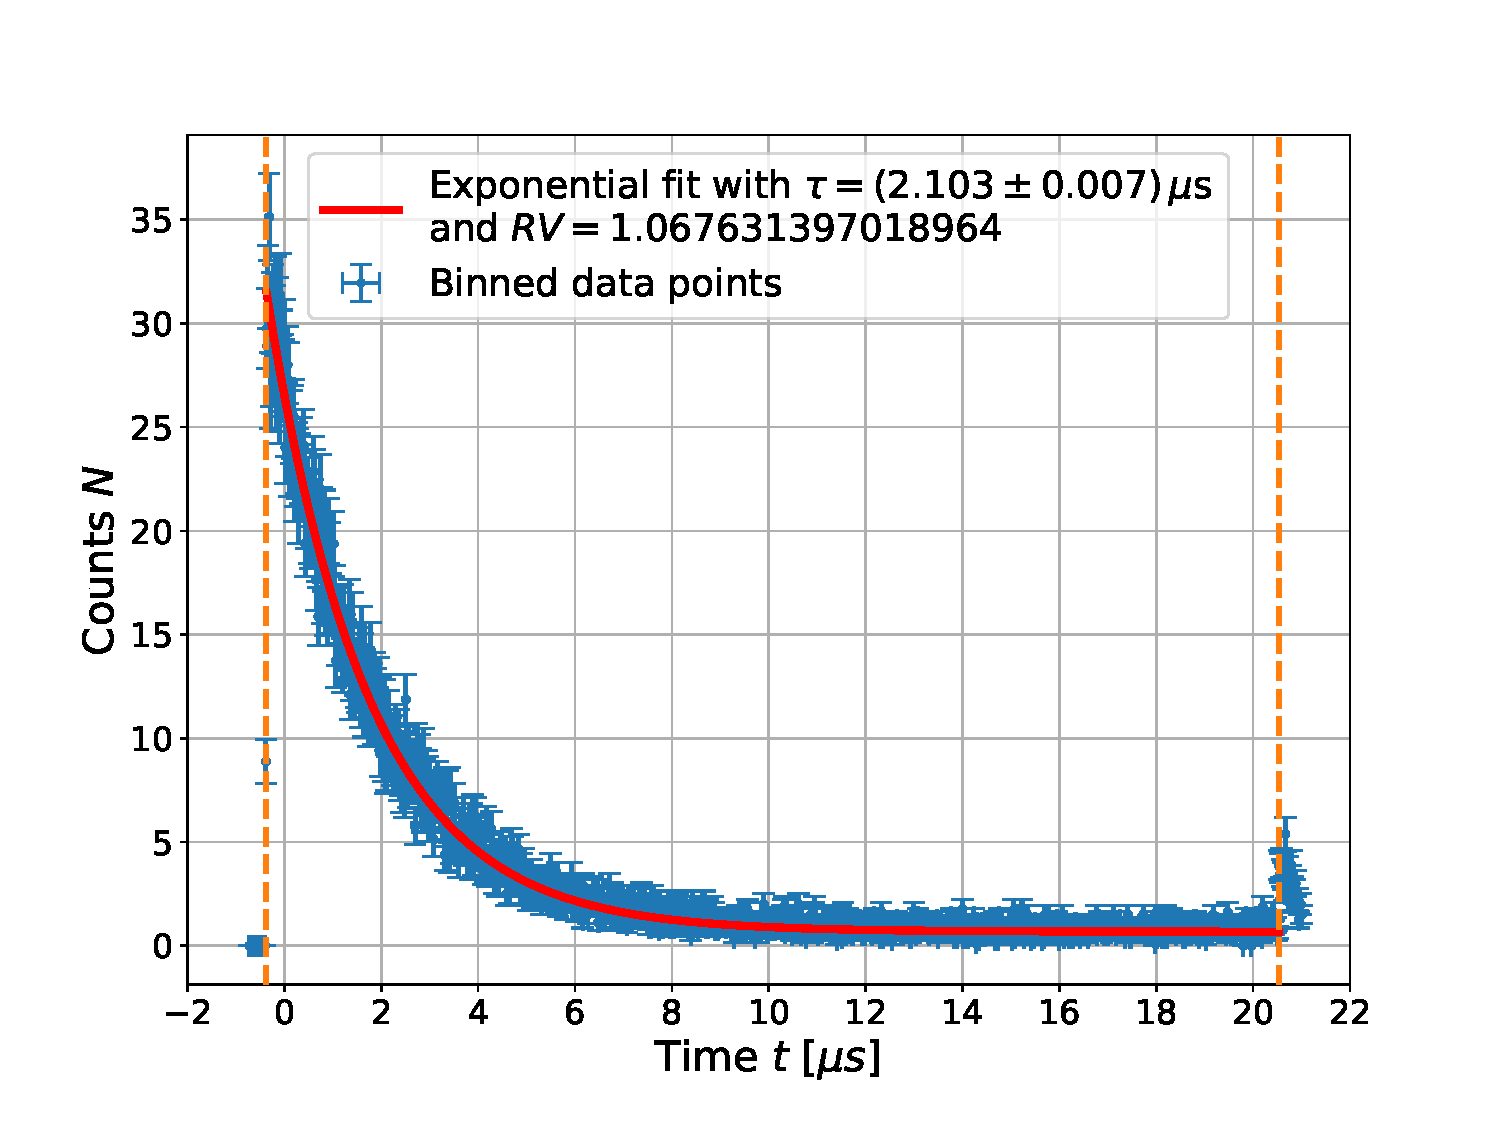
\includegraphics[width=0.8\textwidth]{src/MeanLifetime}
	\caption{This figure shows the measured time spectrum as well as the results of the lifetime measurement of muons.}
	\label{MeanLifetime}
\end{figure}
\noindent As already mentioned in section \ref{MeanLifetimeOfMuons}, the muon decay occurs exponentially, so an exponential fit of the shape
\begin{align} \label{exponential}
N(t)=N_0\cdot\exp\left(-\frac{t}{\tau}\right) + n
\end{align}
\noindent is applied to the binned data points that lie between the two orange, dashed, vertical lines in the diagram in figure \ref{MeanLifetime}.
Since the binned data points, which are outside of this interval, do not have a physical meaning and are irrelevant for the creation of the fit curve.
The resulting fit parameters are
\begin{align*}
N_0 &= 25.84\pm 0.08 \\
\tau &= (2.103\pm 0.007)\,\mu\text{s} \\
n &= 0.678\pm 0.005
\end{align*}
\noindent Here, the parameter $\tau$ corresponds to the mean lifetime of muons.
The comparison of this experimentally determined value with the value provided by the literature in section \ref{MeanLifetimeOfMuons} shows a great difference in the second decimal place.
Both values for the mean lifetime of muons do not coincide, even if you take their standard deviation into account.



\subsection{Angular dependency of muons}

Figure \ref{EnergySpectrum} shows the results of the measurement of the energy loss spectra of the incoming muons at four different zenith angles $\theta$: $0\,$°, $30\,$°, $45\,$° and $75\,$°.
\begin{figure}[H]
	\centering
	\begin{subfigure}[t]{0.495\textwidth}
		\centering
		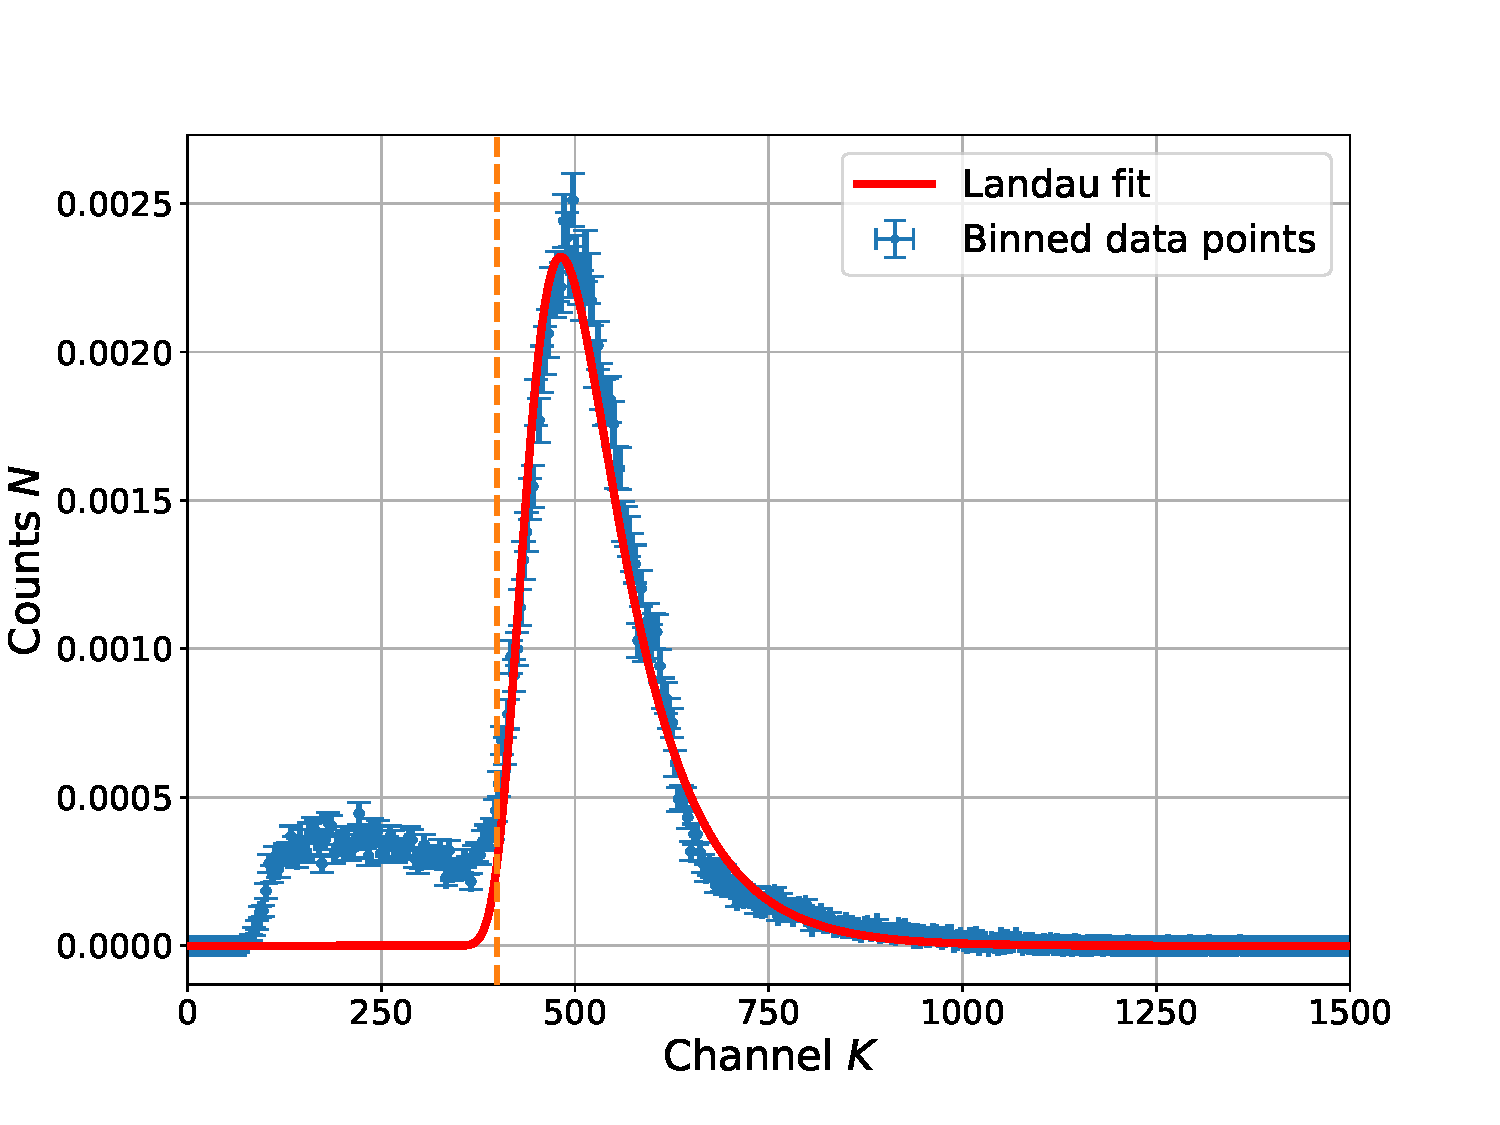
\includegraphics[width=\textwidth]{src/EnergySpectrumAt0Degrees}
		\caption{Energy loss spectrum at $\theta =0\,$°.}
		\label{EnergySpectrumAt0Degrees}
	\end{subfigure}
	\begin{subfigure}[t]{0.495\textwidth}
		\centering
		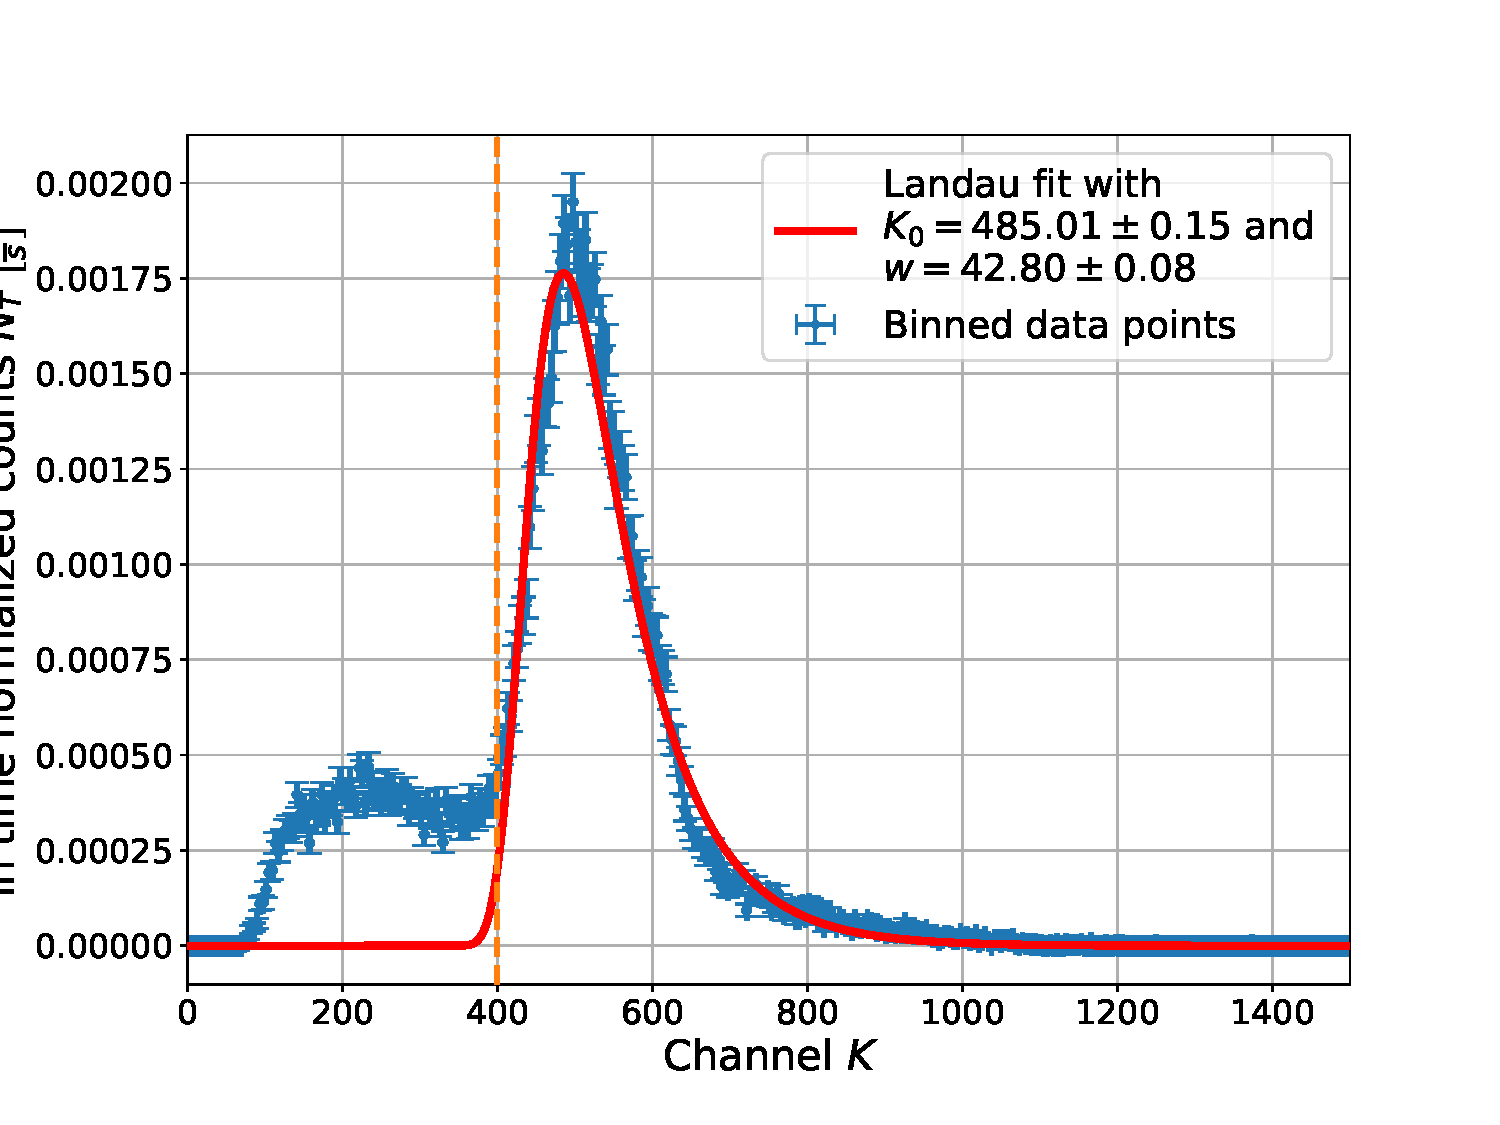
\includegraphics[width=\textwidth]{src/EnergySpectrumAt30Degrees}
		\caption{Energy loss spectrum at $\theta =30\,$°.}
		\label{EnergySpectrumAt30Degrees}
	\end{subfigure}
	\begin{subfigure}[t]{0.495\textwidth}
		\centering
		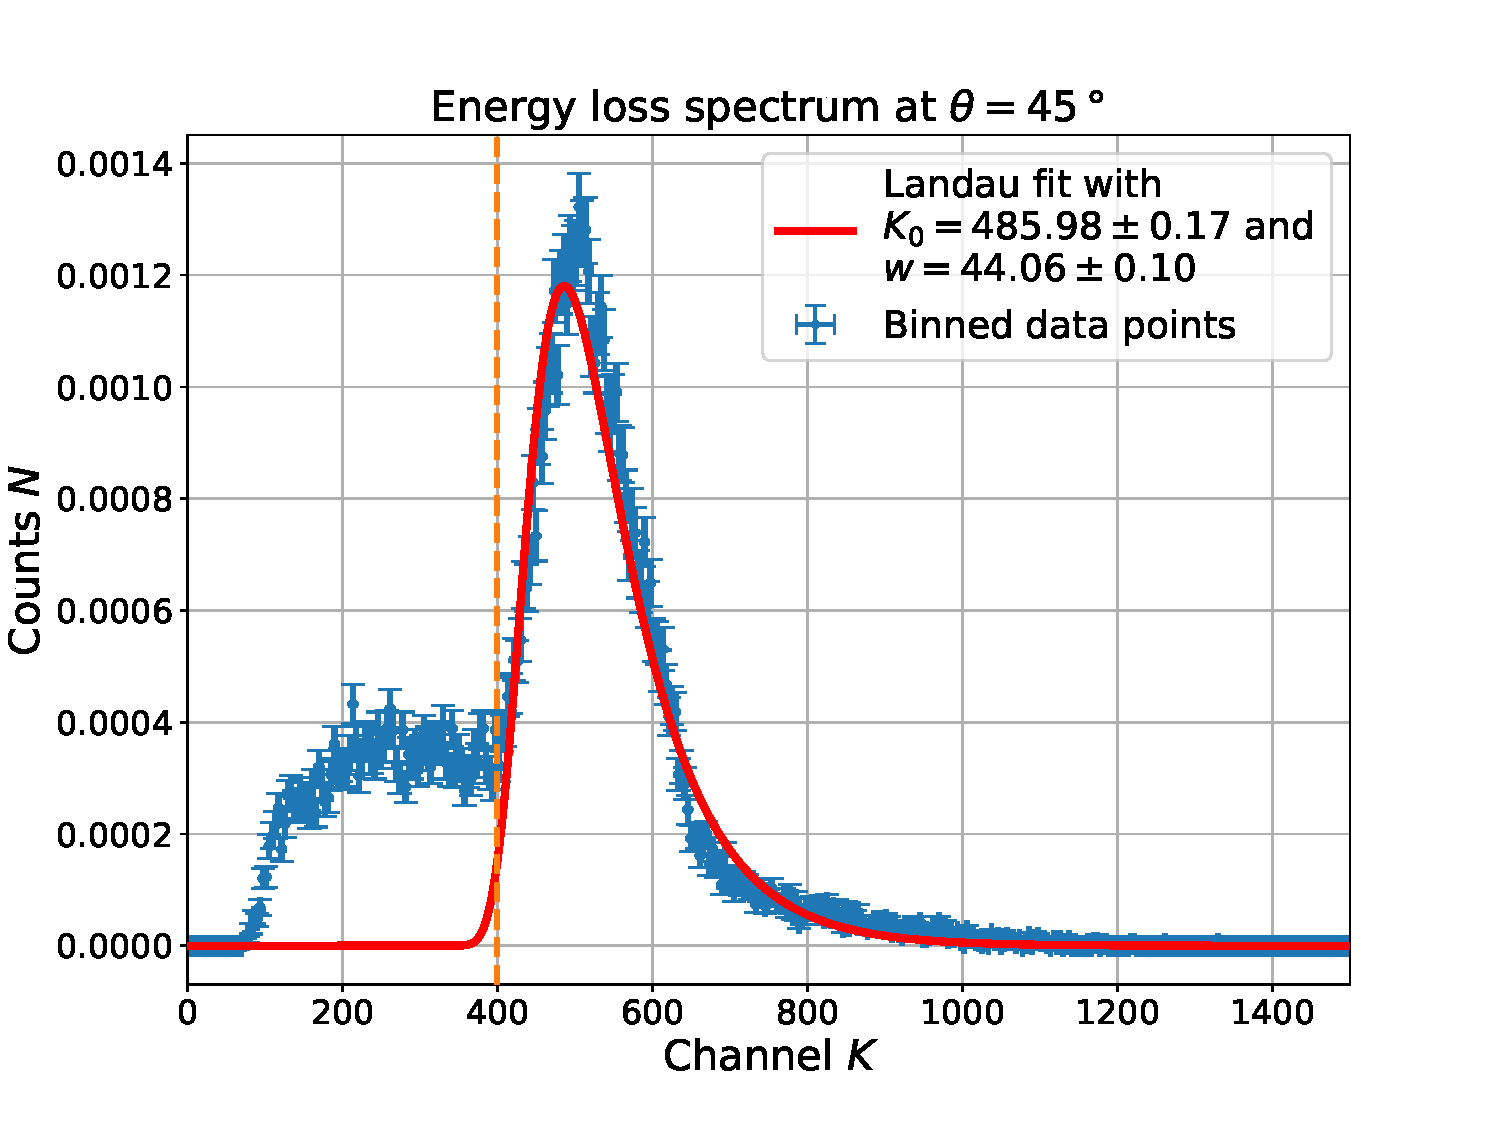
\includegraphics[width=\textwidth]{src/EnergySpectrumAt45Degrees}
		\caption{Energy loss spectrum at $\theta =45\,$°.}
		\label{EnergySpectrumAt45Degrees}
	\end{subfigure}
	\begin{subfigure}[t]{0.495\textwidth}
		\centering
		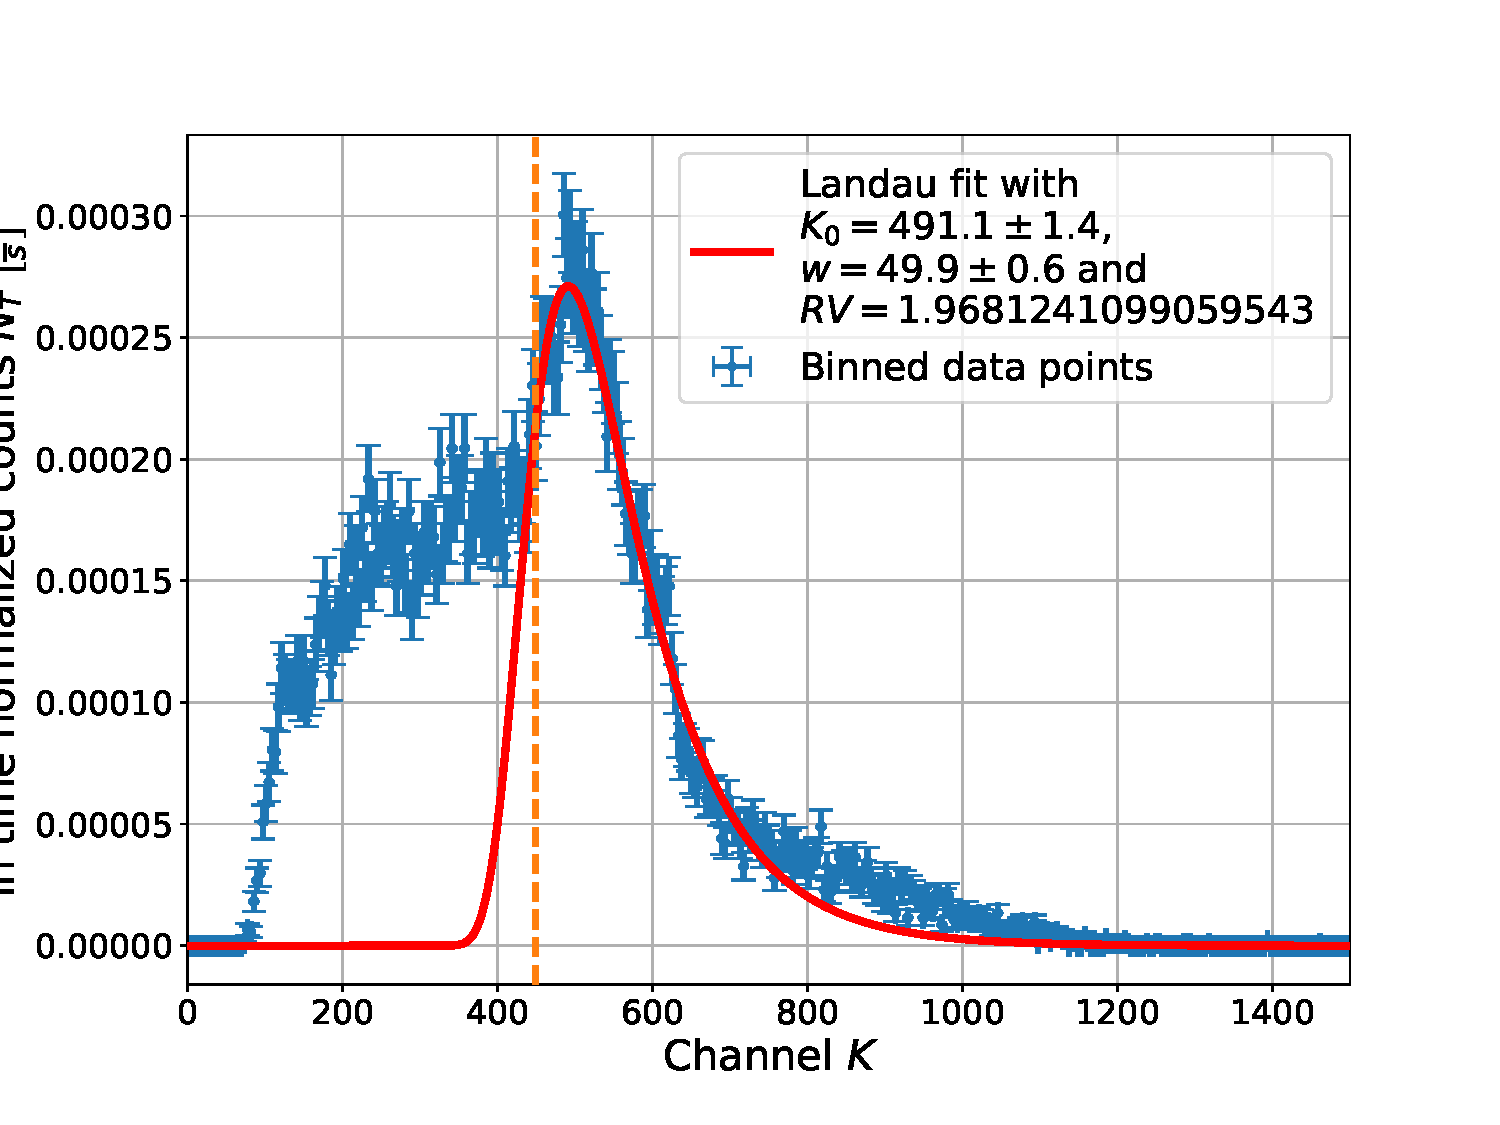
\includegraphics[width=\textwidth]{src/EnergySpectrumAt75Degrees}
		\caption{Energy loss spectrum at $\theta =75\,$°.}
		\label{EnergySpectrumAt75Degrees}
	\end{subfigure}
	\caption{This figure displays four diagrams, which show the energy loss spectrum of the muons at four different zenith angles $\theta$. The channel number $K$ represents the x axis and is proportional to the energy the incoming muons deposits in the detector. On the y axis the counts $N_T$ are shown, which are binned with the factor $b=4$ and normalized in time under the use of the corresponding active measurement time $T$.}
	\label{EnergySpectrum}
\end{figure}
\noindent The data set that is taken from the angle measurement comprises the counts $N_i$ of every energy loss spectrum.
All these counts $N_i$ are binned with the bin factor $b=4$ and under the iterative use of the formula (\ref{Binning}).
Afterwards, the resulting binned counts are normalized in time by dividing with the corresponding active measurement time $T$.
By this means, the counts $N_T$ are calculated.
One needs to point out that the channel number $K$ is related linearly to the energy, which the incoming muons looses and deposits in the detector by travelling through it.
From section \ref{PeakEnergyLossDistribution} it is known that the energy deposition of an incoming muon in the detector can be described by a Landau distribution.
As this function is defined by a complex integral, an approximation of the shape
\begin{align} \label{LandauDistribution}
p(x)\approx\frac{A}{\sqrt{2\pi}}\cdot\exp\left[-\frac{1}{2}\cdot\left(\frac{\left(x-K_0\right)}{w}+e^{-\frac{(x-K_0)}{w}}\right)\right]
\end{align}
\noindent is used to fit the binned data points in each of the four diagrams in figure \ref{EnergySpectrum}.
Here, $A$ is the Amplitude, $K_0$ is the position of the maximum and $w$ is the width of the Landau distribution.
In the curve fitting process, only the binned data points on the right side of the orange, dashed, vertical lines are taken into account.
All the data points on the left side of this lines are ignored, because they can be identified as background noise.
Each Landau fit is illustrated in the corresponding diagram in figure \ref{EnergySpectrum}.
The resulting fit parameters can be gathered from the table \ref{LandauFitParameters}.
\begin{table}[H]
	\centering
	\caption{This table shows the parameters for the Landau fits of all four energy loss spectra in figure \ref{EnergySpectrum}.}
	\begin{tabular}{|c|c|c|c|}
		Zenith & Amplitude $A$ $\left[\frac{1}{\text{s}}\right] $ & Position $K_0$ of & Width $w$ \\
		angle $\theta$ &  & the maximum &  \\
		\hline
		$0\,$° & $(9.59\pm 0.02)\cdot 10^{-3}$ & $481.61\pm 0.13$ & $41.56\pm 0.08$ \\
		\hline
		$30\,$° & $(7.29\pm 0.02)\cdot 10^{-3}$ & $485.01\pm 0.15$ & $42.80\pm 0.08$ \\
		\hline
		$45\,$° & $(4.879\pm 0.015)\cdot 10^{-3}$ & $485.98\pm 0.17$ & $44.06\pm 0.10$ \\
		\hline
		$75\,$° & $(1.120\pm 0.010)\cdot 10^{-3}$ & $491.1\pm 1.4$ & $49.9\pm 0.6$ \\
	\end{tabular}
	\label{LandauFitParameters}
\end{table}
\noindent As already mentioned in section \ref{PeakEnergyLossDistribution}, the position $K_0$ of the maximum displays the most probable energy deposition, which is a qualitative hint for the total kinetic energy of the incoming muon.
If you look at the four $\theta$ and $K_0$ values in the first and third column in table \ref{LandauFitParameters}, you obtain $K_0^\text{0\,°}<K_0^\text{30\,°}<K_0^\text{45\,°}<K_0^\text{75\,°}$.
This means that the larger the zenith angle is set, the greater the measured energy loss becomes.
So, you can measure high-energy muons by choosing a great zenith angle.

Now, the count rate $R$ for each of the four energy loss spectra is calculated.
In order to consider only the counts of the muons with a particular energy characteristic, the count rate $R$ is defined as the sum over all measured counts in the $\pm w$ interval around the position $K_0$ of the maximum of a Landau distribution, which is divided afterwards by the corresponding active measurement time $T$.
If you plot the resulting count rates $R$ against the corresponding zenith angles $\theta$ and apply a squared cosine fit of the shape
\begin{align} \label{KosinusQuadrat}
h(x)=A\cdot\cos^2\left(\frac{\pi}{180\,\text{°}}\cdot\theta\right)
\end{align}
\noindent to the data points, you get the diagram in figure \ref{AngularDependency}.
\begin{figure}[H]
	\centering
	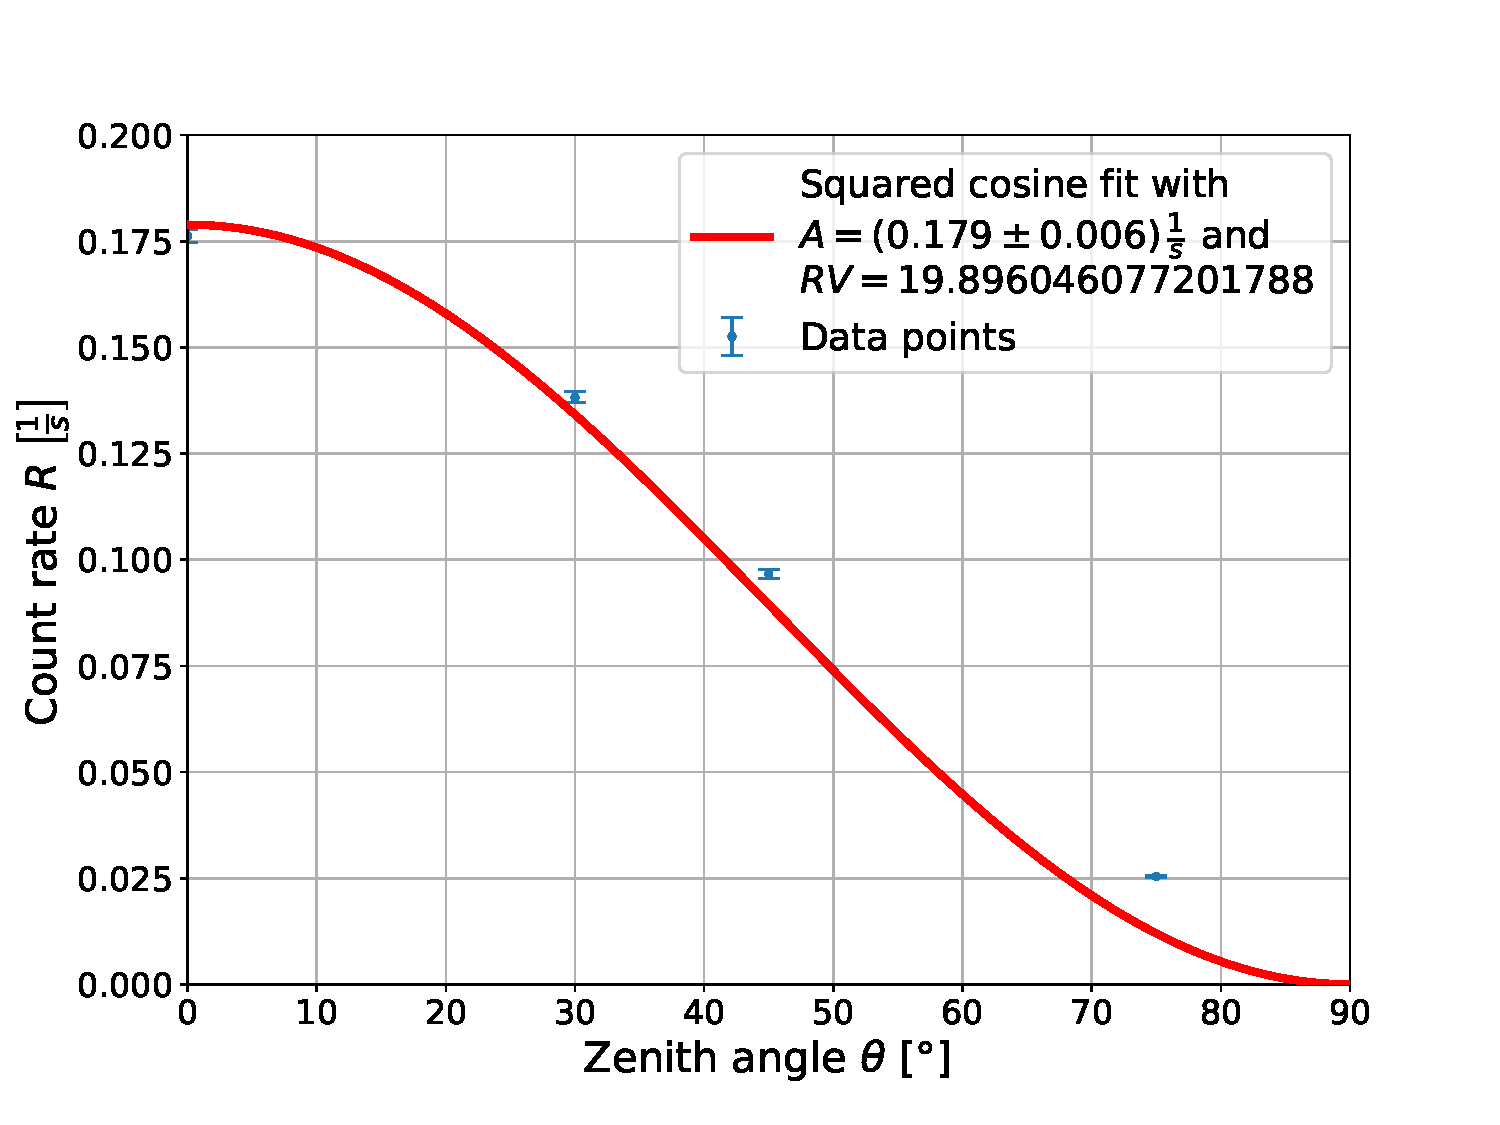
\includegraphics[width=0.8\textwidth]{src/AngularDependency}
	\caption{This figure shows a diagram, which elucidates the angular dependency of the muon count rate $R$. Therefore, the zenith angle $\theta$ is displayed on the x axis. The count rate $R$ represents the y axis and is a sum over all measured counts in the $\pm w$ interval around the position $K_0$ of the maximum of a Landau distribution, which is divided afterwards by the corresponding active measurement time $T$.}
	\label{AngularDependency}
\end{figure}
\noindent Here, $A$ is the amplitude and a constant factor.
The value of this fit parameter can be gathered from the legend of the diagram.
It is observable that the squared cosine fit curve fits well with the data points.
This result corresponds to the theoretical predictions in section \ref{DependencyZenithAngle}.